\documentclass[notitlepage, a4paper, 12pt]{report}

\usepackage[utf8]{inputenc}
\usepackage[T1]{fontenc}
\usepackage{ragged2e}
\usepackage{geometry}
\usepackage{graphicx}
\usepackage{setspace}
\usepackage{hyperref}
\graphicspath{{.}}


\begin{document}

% ########## TITLE PAGE
\pagestyle{empty}
\centering


\includegraphics[scale=0.75]{Sciences_SU}
\\
\vspace{20mm}
\rule{\textwidth}{0.4pt}
\huge \bf
Carnet de bord :

Waterpixels, des super-pixels respectant les contours des objets dans les images
\rule{\textwidth}{0.4pt}
\\
\vspace{20mm}
\normalsize Auteur : Mathias VELO
\\
\vspace{5mm}
2 avril 2021
\\
\vspace{40mm}
\begin{flushright}
\emph{Encadrant: Isabelle BLOCH}
\end{flushright}

\newpage

% ########## START
\setcounter{page}{1}
\pagestyle{plain}

\begin{flushleft}

\section*{\underline{Introduction}}

Mon sujet de recherche porte sur l'implémentation d'une méthode de segmentation d'image nommée \emph{waterpixels}.
\newline
\newline
Ces superpixels, ou waterpixels, permettent de partitionner l'image de façon assez régulière, en obtenant une détection de contours très précise.
\newline
\newline
La détection de contours est une première étape dans un pipeline de traitement de l'image, pouvant servir entre autres à des applications de vision par ordinateur, dont la reconnaissance faciale et la robotique.
\newline
\newline
Cette première étape de segmentation doit donc être efficiente en temps de calcul, car le résultat de la segmentation n'est pas une fin en soi, mais une première étape vers d'autres traitements successifs.
\newline
\newline
Afin de répondre à cette contrainte, j'ai décidé d'implémenter le code en C++, et de me servir d'OpenCL afin de massivement paralléliser les calculs sur GPU. À défaut de pouvoir me servir de la carte graphique pour certains algorithmes, j'ai fais usage du multithreading sur CPU.

\section*{\underline{Mots clés}}

\fbox{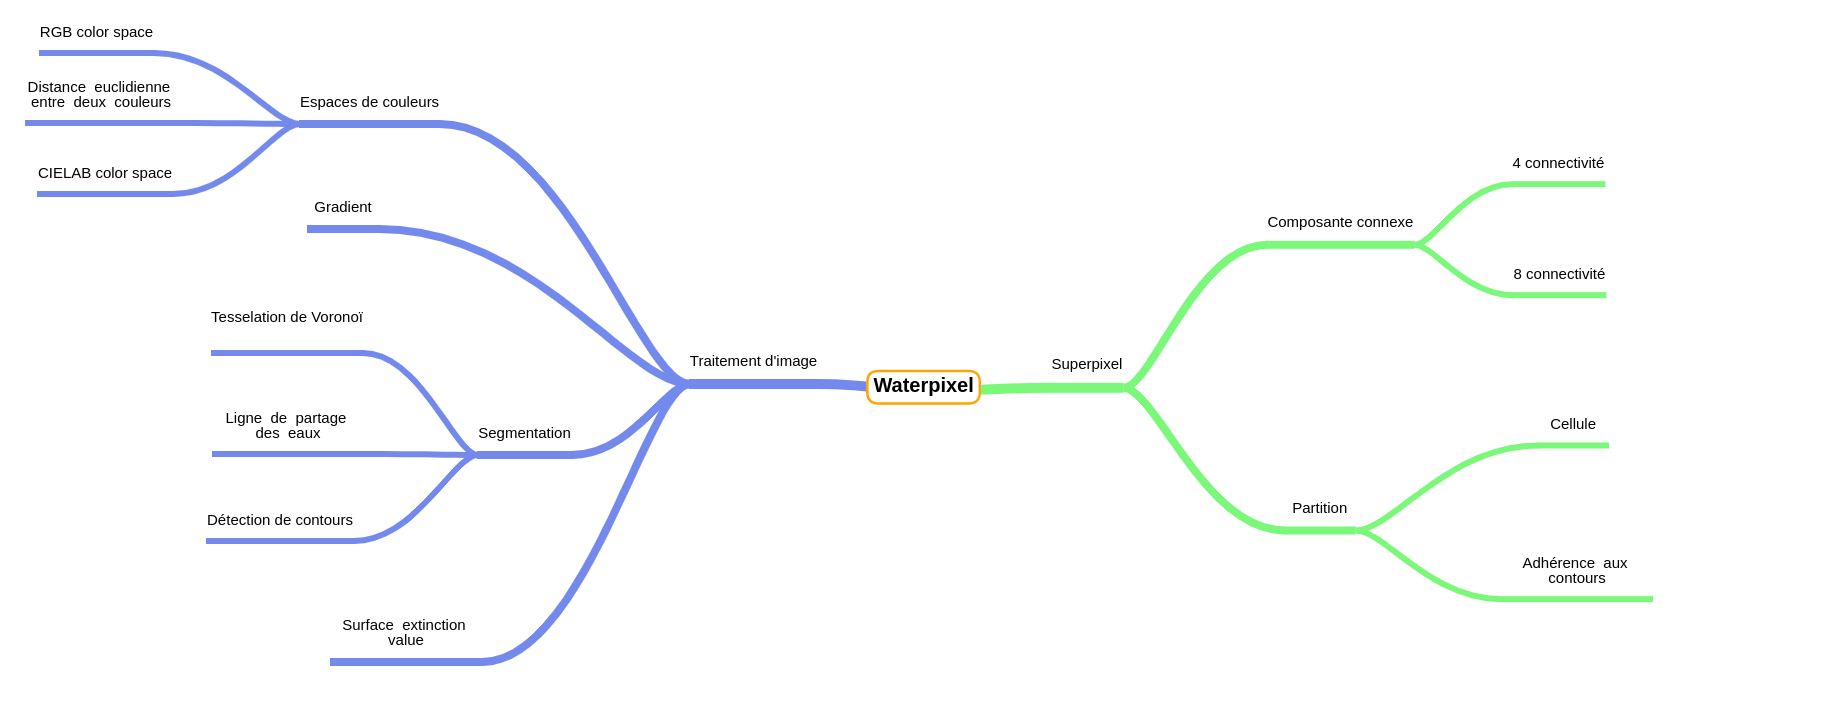
\includegraphics[scale=0.25]{mindmap}}

\section*{\underline{Recherche documentaire}}

Mes recherches se sont principalement portées sur des aspects techniques, tels que la découverte de l'outil OpenCL[4][5][6] pour les besoins du projet, et la manière dont on passe d'un espace de représentation des couleurs à un autre (espace RGB vers LAB)[2].
\newline
\newline
Je me suis bien évidemment servis du document de référence[1] sur les waterpixels fournis par mon encadrante, et ai consulté une ressource externe sur les "extinction values"[3] en citation de ce document.
\newline
\newline
Pour la conception de l'IHM avec le framework Qt, je me suis simplement servis de la documentation officielle en ligne, à cette adresse : \url{https://doc.qt.io/qt-5/qtgui-module.html}, laquelle listant toutes les classes d'interface utilisateur, et renseignant la manière dont il faut se servir de telle ou telle classe.
\newline
\newline
Ce projet a aussi été l'occasion pour moi de découvrir un algorithme de segmentation d'image très utilisé : la segmentation par ligne de partage des eaux.\newline
Produire cet algorithme était la partie la plus complexe pour moi.\newline
Mes premiers algorithmes étaient inutilement compliqués, et c'est à partir de la troisième version que j'ai obtenu les résultats attendus.\newline

\section*{\underline{Bibliographie}}

[1] Vaïa Machairas, Matthieu Faessel, David Cárdenas-Peña, Théodore Chabardes, Thomas Walter, et
al.. Waterpixels. IEEE Transactions on Image Processing, Institute of Electrical and Electronics
Engineers, 2015, 24 (11), pp.3707 - 3716. 10.1109/TIP.2015.2451011. hal-01212760

\vspace{7mm}

[2] “Les espaces de couleur RVB et Lab,” Accessed on: Feb. 22, 2021. [Online]. Available: \url{http://www.tsi.enst.fr/pages/enseignement/ressources/beti/RVB_ou_LAB/html/colorspace.html}

\vspace{7mm}

[3]	A. G. Silva et R. d A. Lotufo, « New Extinction Values from Efficient Construction and Analysis of Extended Attribute Component Tree », in 2008 XXI Brazilian Symposium on Computer Graphics and Image Processing, oct. 2008, p. 204‑211, doi: 10.1109/SIBGRAPI.2008.8.

\vspace{7mm}

[4] David Gohara. "Episode 1 - Introduction to OpenCL", YouTube, June. 18, 2013 [Video file]. Available: https://www.youtube.com/watch?v=QA483lIvL-4. [Accessed: Sat. 20, 2021].

\vspace{7mm}

[5] David Gohara. "Episode 2 - OpenCL Fundamentals", YouTube, June. 18, 2013 [Video file]. Available: https://www.youtube.com/watch?v=e-2bTxKuS2U. [Accessed: Sat. 20, 2021].

\vspace{7mm}

[6] David Gohara. "Episode 3 - Building an OpenCL Project", YouTube, June. 18, 2013 [Video file]. Available: https://www.youtube.com/watch?v=yAz9Kj6zRcA. [Accessed: Sat. 20, 2021].

\section*{\underline{Évaluation des sources}}

Source \textnumero{2} :\newline

Source trouvée avec une simple requête de la forme "RGB to LAB color space" sur le moteur de recherche Google, aussi bien en français qu'en anglais.

Je ne connais pas la date de publication de cette page web, mais il s'agit de calculs mathématiques, dont la validité est intemporelle.
L'information est pertinente, va droit au but en expliquant comment la conversion s'effectue dans un sens comme dans l'autre (RGB vers LAB et LAB vers RGB).
Cette page est une ressource éducative dont la propriété intellectuelle appartient à l'école Télécom Paris, cette source est donc de confiance.
\newline

Source \textnumero{3} :\newline

Source datant de 2008, et trouvée en citation dans le document de référence[1] pour mon sujet traitant des waterpixels.
Il s'agit d'un document scientifique de recherche, publié par des chercheurs, donc pertinent.
Il m'a servis afin de comprendre la signification exacte du terme \emph{surface extinction values}, peu importe la date de publication, je souhaitais simplement comprendre le concept derrière ce terme, afin de pouvoir continuer l'implémentation du projet.
\newline

Source \textnumero{4} \textnumero{5} \textnumero{6} :\newline

Tutoriels youtube traitant d'OpenCL.\newline
Comprendre son fonctionnement et sa prise en main.\newline
Ces vidéos datent de 2013, à cette date OpenCL 1.2 était déjà disponible depuis 2 ans, la version 1.2 étant la version la plus utilisée aujourd'hui et reste le coeur des fonctionnalités d'OpenCL 3.0 qui est sortit en avril 2020. De plus, je suis un débutant et nouvel utilisateur, donc je ne me sers pas encore d'outils très avancés disponibles dans la version 2.0 ou 3.0.
Ces leçons m'ont donc tout à fait convenu.
L'auteur David Gohara est un biochimiste ayant fait un postdoc à Harvard (d'après son linkedin).
Grâce à ces vidéos j'ai pu faire un simple hello world en langage C, que j'ai par la suite encapuslé dans une classe C++ réutilisable.

\end{flushleft}


\end{document}
